% ======================= CHAPTER V =======================
\chapter{Analysis and Discussion}\label{ch:discussion}

\section{Hardware Development}
 The hardware development of MAGIC is relatively simple, considering the components used and the way they are assembled. However, several challenges related to operation in hazardous environments, portability, and robustness appear during the process.
 \newp
 The design of the resonant coils is a critical aspect of the hardware development, and scaling the system in terms of current, área and turns is not trivial. The trade-offs between size, weight, and performance must be carefully considered to achieve an optimal design that meets the requirements of particular underground applications.
 \newp
    Additionally, the choice of materials and construction techniques must take into account the environmental conditions in which the system will operate, including temperature variations, moisture, and mechanical stresses.
\newp
Loop antennas developed for MAGIC have an equilibrated performance considering the size and weight of the system. The total weight of the resonant coil is around 2 kg, which is relatively light for a TTE communication system, but still provides a good performance in terms of the intensity of the magnetic field generated and received. The design of a circular coil permits a uniform magnetic field distribution, and a maximum of magnetic flux at the receiver if it's on the central axis of the structure. Furthermore, this design allows for direct scaling of the system if greater communication distances are desired. Due to the natural trade-off between the current flowing through the coil and the number of turns, the simplest way to scale the system is by increasing the diameter of the antennas. This is because a greater number of turns means the winding conductor must be longer, and therefore the actual resistance of the coil increases, and the amplifier can deliver less current to the coil. However, increasing the diameter of the coil also means more conductive material and therefore more resistance; it's the best way to scale the system, considering also that a larger area means more magnetic flux at the receiver.

\subsection{Topology at Transmitter and Receiver}

At the beginning of the development of MAGIC, the series configuration between the coil and tuning capacitor was used at the transmitter and the receiver due to its simplicity and symmetrical configuration to permit bidirectional communication. However, it is interesting to analyze other configurations that could be more efficient in terms of power transfer and signal reception.
\newp
Here is a simulation of all four configurations of series and parallel at the transmitter and receiver, considering the same coil and tuning capacitor for all the cases. The results in terms of the transfer function are given in the following figure.

\begin{figure}
    \centering
    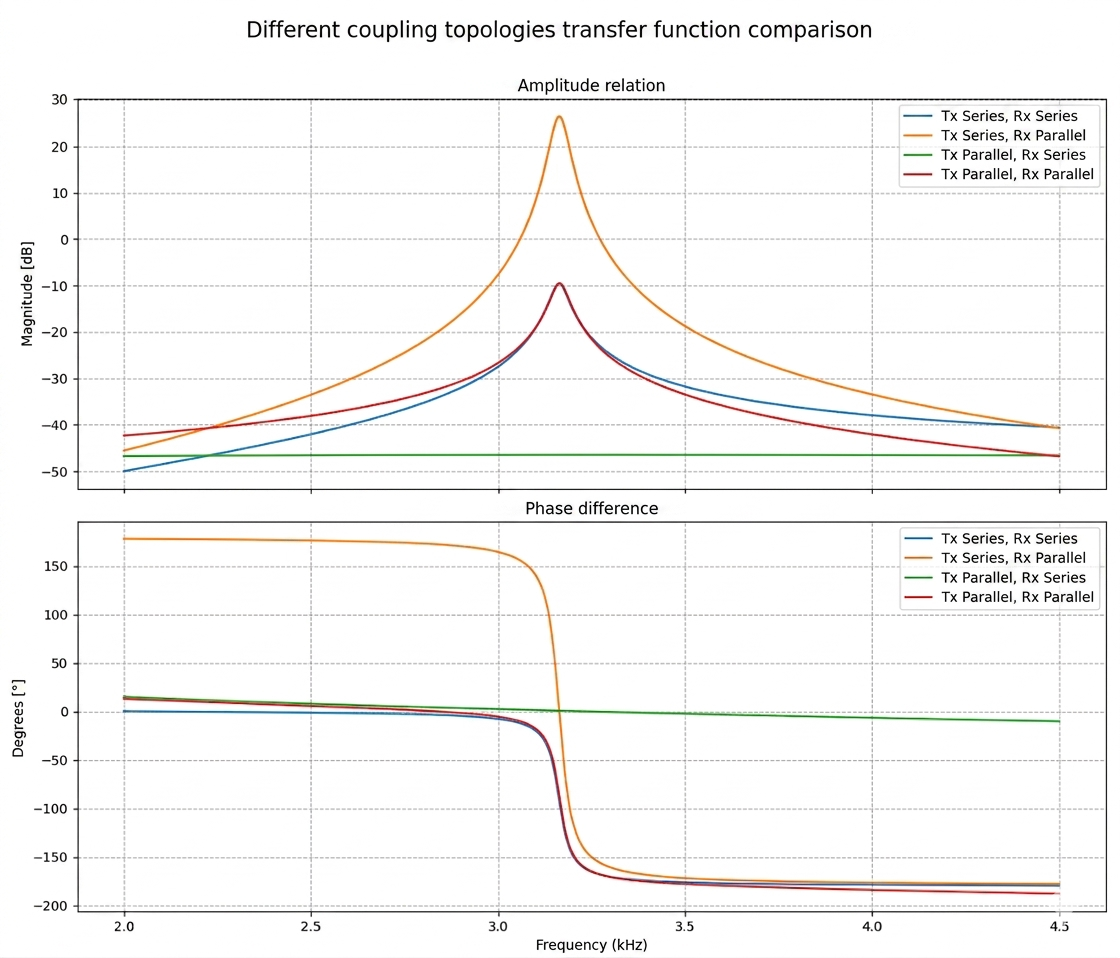
\includegraphics[width=0.9\textwidth]{img/topo.png}
    \caption{Transfer function for different configurations of series and parallel at the transmitter and receiver.}
    \label{fig:transfer-function_4}
\end{figure}

It's clear that the actual configuration used in MAGIC works, but it is not the most efficient in terms of power transfer. Regarding the transmitter, the parallel configuration is suboptimal due to the high impedance of the circuit. The impedance of a parallel LC circuit at resonance is:

\begin{equation}
    Z_{paralelo} = \frac{R + j\omega L}{1 - \omega^2 LC + j\omega RC}
\end{equation}

Where R is the resistance of the coil, L is the inductance of the coil, C is the capacitance of the tuning capacitor, and $\omega$ is the angular frequency. At resonance, where $\omega^2 LC = 1$, the impedance becomes:

\begin{equation}
    Z_{paralelo} \approx \frac{L}{RC} = Q^2 R
\end{equation}

Where Q = $\frac{1}{R}sqrt{frac{L}{C}}$ is the quality factor of the coil. This means that the impedance of the parallel configuration at resonance is much higher than the resistance of the coil, so less current can be delivered to the transmitter coil.

On the other hand, the series configuration at the transmitter has an impedance at resonance of:
\begin{equation}
    Z_{serie} = R + j \left( \omega L - \frac{1}{\omega C} \right)
\end{equation}

At resonance, the impedance becomes:
\begin{equation}
    Z_{serie} = R
\end{equation}

So the series configuration at the transmitter allows for maximum current to be delivered to the coil. Actually, in this case the resistance of the transmitter is only 3 $\Omega$, so the amplifier can deliver a maximum current of around 3 A.

Regarding the receiver, the parallel configuration is more efficient in terms of signal reception. Although it has higher impedance, a parallel LC circuit works as a pure resonator, meaning the energy stored in the coil is transferred to the capacitor and then back to the coil, and so on. That results in a higher voltage across the capacitor, which is where the signal is measured; this voltage depends on the quality factor. Additionally, the audio interface's impedance is closer to the impedance of the parallel configuration, which is beneficial for signal transfer. On the other hand, the series configuration at the receiver has a lower voltage; it only corresponds to the voltage drop across the resistance of the circuit, but isn't a voltage amplification mechanism like the parallel configuration. For that reason, the parallel configuration at the receiver is more efficient in terms of signal reception.
\newp
A short test was made to compare the performance of parallel and series configurations at the receiver, using the same coil and tuning capacitor for both cases. Here is a spectrum plot of the noise captured by the receiver at Cerro Calán in both configurations, shown in figure \ref{fig:receiver-configurations}.

\begin{figure}
    \centering
    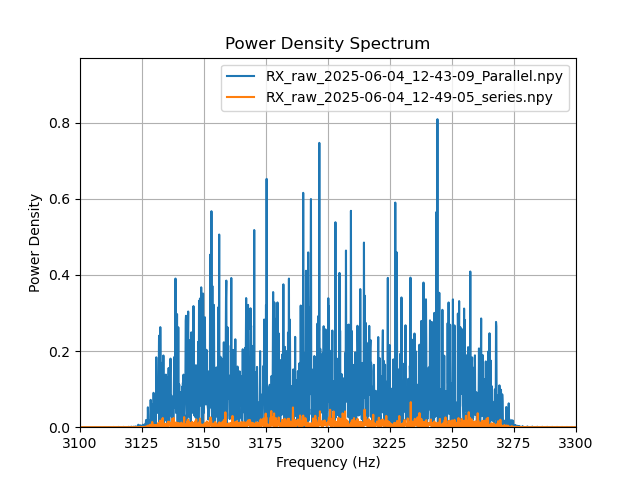
\includegraphics[width=0.9\textwidth]{img/Noise_p_s.png}
    \caption{Spectrum of noise captured by the receiver in parallel and series configuration.}
    \label{fig:receiver-configurations}
\end{figure}


The results showed that the parallel configuration at the receiver provided a stronger signal compared to the series configuration, confirming the theoretical analysis.
\newp
Measuring communication performance in terms of SNR, correlation peak and SER the results are:

\begin{table}
    \centering
    \begin{tabular}{c|c|c|c}
        Configuration of Receiver & mean SNR (dB) & Max Correlation Peak & SER (\%) \\
        \hline
        Series & 6.47 & 144.18 & 0.0 \\
        Parallel & 7.42 & 19.25 & 0.0 \\
    \end{tabular}
    \caption{Performance comparison between series and parallel configuration at the receiver.}
    \label{tab:receiver-performance}
\end{table}

The results show that the parallel configuration at the receiver provides a slightly higher SNR compared to the series configuration. Considering the LC tank's amplifies both noise and signal, this result could be a coincidence. However, a parallel configuration demonstrates a higher mean correlation peak that is useful to take advantage of the dynamic range of the audio interface.

\subsection{Interference and electromagnetic compatibility}

Interference was a significant challenge during the hardware development of MAGIC. Primarily, the noise sources were not well known, and it was through testing that they began to appear. For example, at the beginning, when MAGIC didn't have its own power supply (battery) and the module was to be connected to the power grid, the noise from the power lines made the difference between detecting the signal or not at low SNR. In Figure \ref{fig:noise-grid}, a measure of the noise captured by the receiver when the module is connected to the power grid is shown, considering two measures for each configuration. This test was made in the Millimeter Wave Laboratory of the Universidad de Chile.

\begin{figure}
    \centering
    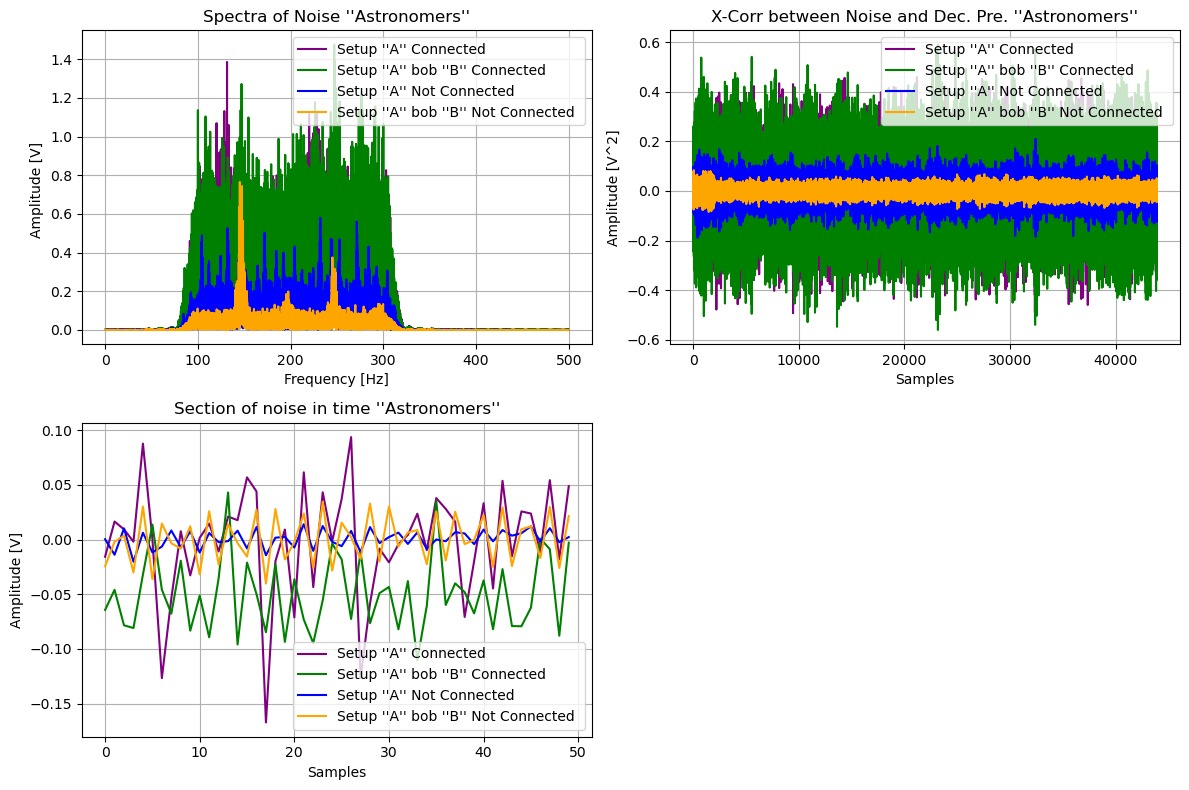
\includegraphics[width=0.9\textwidth]{img/noise.jpeg}
    \caption{Spectrum of noise captured by the receiver when the module is connected to the power grid.}
    \label{fig:noise-grid}
\end{figure}

It is clear that when the MAGIC central module is connected to the power grid, i.e., the amplifier is powered on. The noise level increases significantly, and also the correlation peaks.
\newp
To mitigate this issue, the decision was to use a battery as the power supply for the module and switch the power of the amplifier on only during the transmission of the signal.
\newp
Another noise source, also coming from the power grid, appeared when the laptop was connected to the power grid. Additionally, noise from the proper laptop was also a problem; if it was too close to the coil, there could be false positives in the correlation. It was necessary to define a minimum distance free of electronic devices around the coil to avoid this kind of interference. For future versions of MAGIC, it would be interesting to implement a more robust shielding of the receiver path from the coil to the audio interface, using high-quality audio cables and connectors, while also keeping a proper grounding of the system.


\section{Software development}

There are several aspects to discuss in the software development of MAGIC. First, the choice of modulation scheme (M-FSK) was accured, other modulation schemes that depend on phase like PSK (Phase Shift Keying) or QAM (Quadrature Amplitude Modulation) could not work well considering the naturally dispersive system and changing conditions. Some signal proccessing techniques, including filtering and error correction coding generate that MAGIC works propertly and others, such as decimation, proved counterproductive due to the implementation of the algorithm.

\subsection{Encoding and Symbol Mapping}\label{subsec: Analysis-codification}

The choice of extended ASCII is a consequence of available bandwidth. Depending on the symbol duration, the spectral difference between symbols is defined to maintain orthogonality, as it was explained in section \ref{subsec: ortogonality}, the minimum spectral distance between symbols is 2 $Hz$. As the spectral channels of the FFT at the demodulator have the same width, it is proper to define symbol frequencies, leaving an empty spectral channel between symbols to avoid leakage if the symbols generated don't match exactly with the spectral channels of the FFT. For that reason, we can distribute a maximum of $\sim$112 symbols considering an analog bandwidth of 450 $Hz$.
\newp

Furthermore, considering that there are harmonics in the electrical grid within the band, the space reduces significantly. For example, if we defined a flagged band of 20 $Hz$ around every even or odd harmonic, 270 $Hz$ of the bandwidth is available, and to have more than $\sim$ 67 characters, we have to encode two symbols per character, which is why our bitrate is 8 bps.
\newp
If the encoding scheme changes to, for example, a custom dictionary with 64 characters and a single symbol per character, the bitrate could be increased to 12 bps (the symbol duration is the same) and the char rate could double. This has another benefit that is related to error correction capability. As it was explained in section \ref{subsec: error_correction_code}, the error correction code implemented is based on Reed-Solomon coding, which is a block code capable of correcting half of the parity symbols, and due to the encoding scheme, this translates to correcting a number of characters equal to one-quarter of the parity symbols. Now, if every character is encoded by a single symbol, the error correction code can correct a number of characters equal to half of the parity symbols, i.e, twice the current error correction capability. However, the implementation of a custom dictionary has the cost of reducing the number of characters available.

\newp
To avoid leakage between symbols, it´s necessary to demonstrate that the variability of frequency of the generated tones is lower than the spectral distance between symbols. In Figure \ref{fig:variability}, the variability of a generated tone by the audio interface is shown for a defined amount of time.

\begin{figure}
    \centering
    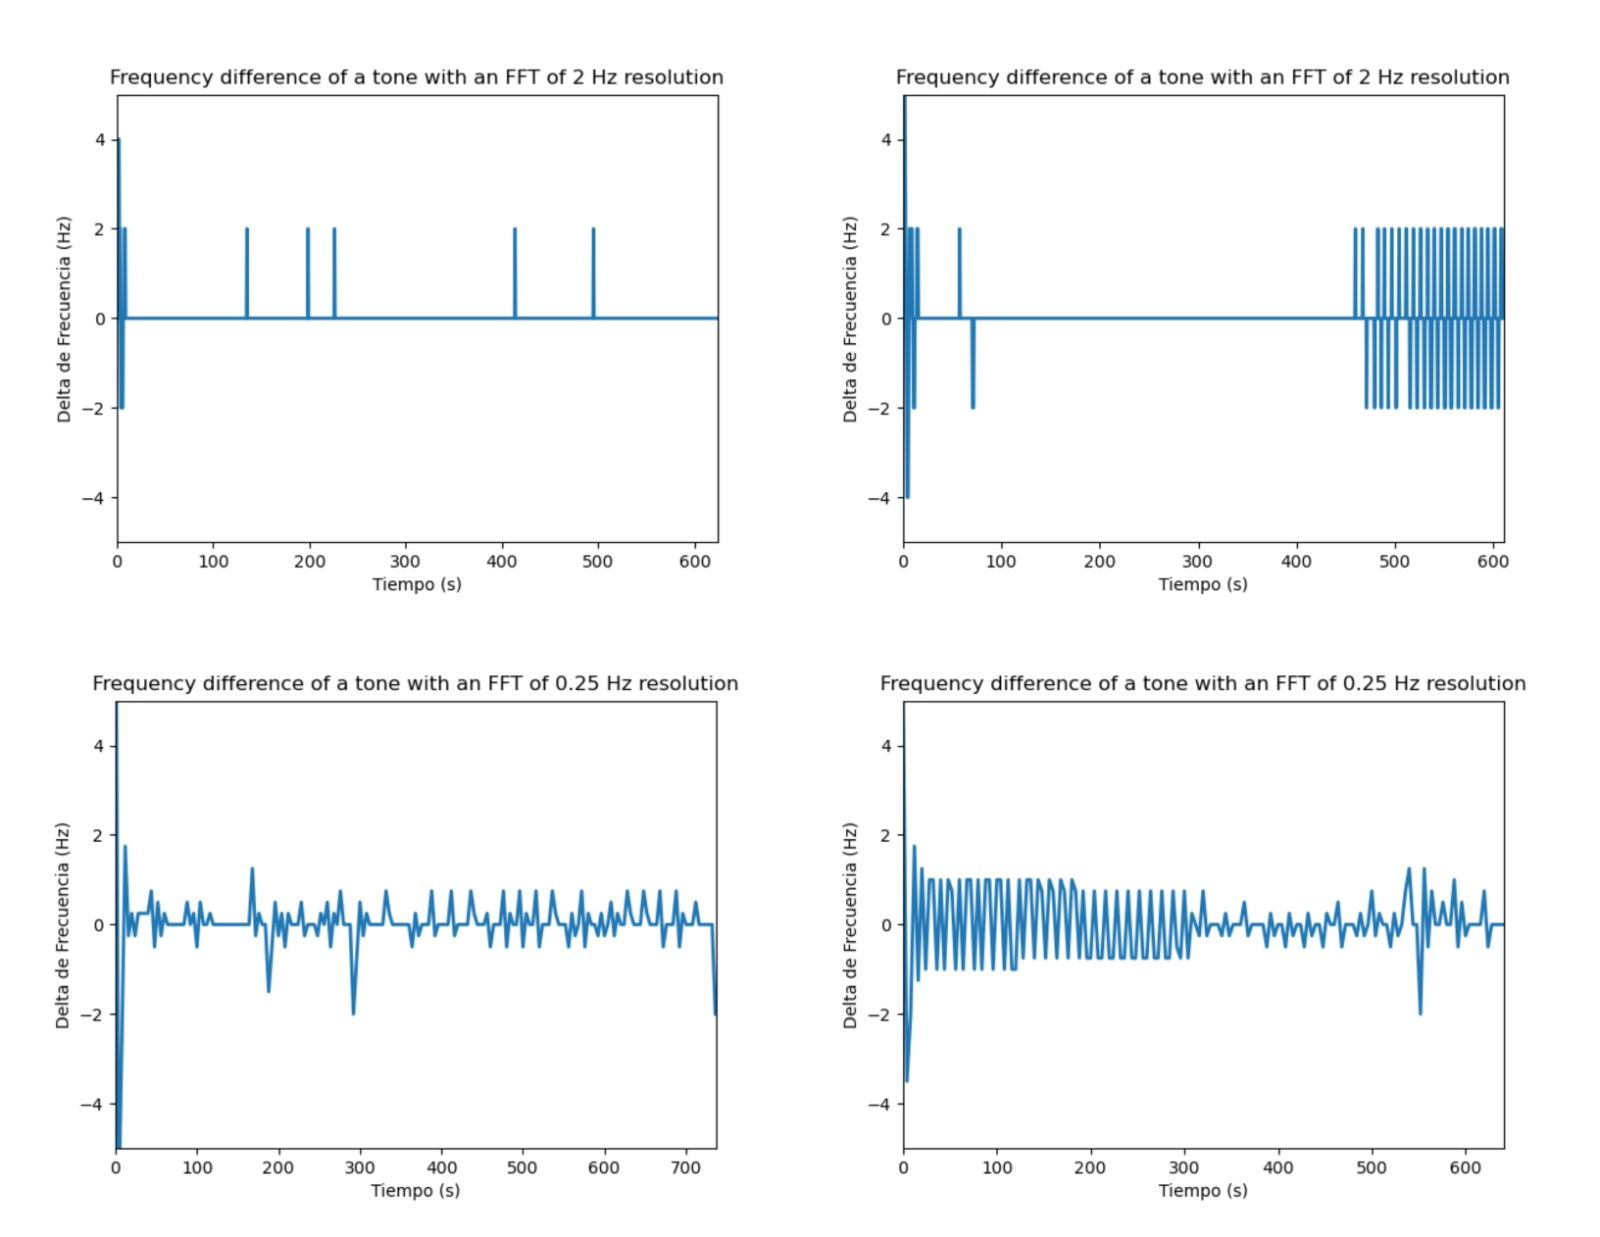
\includegraphics[width=0.9\textwidth]{img/variability.jpeg}
    \caption{Variability of a generated tone by the audio interface for a defined amount of time.}
    \label{fig:variability}
\end{figure}

In the upper left section of figure \ref{fig:variability}, the variability of the spectral peak considering a FFT resolution of 2 $Hz$, like the one used in the demodulator, it's clear that sometimes the peak moves for a little time to the adjacent spectral channel, but does not invade the spectral channel of the adjacent symbol. In the upper right section, the audio interface was heated to induce more variability. At the bottom left section is shown the variability of the spectral peak considering a FFT resolution of 0.25 $Hz$, the peak looks more unstable, but the variations of frequency are close to the FFT resolution, which is good enough. Finally, at the bottom right section, the variability of the spectral peak is shown, considering a FFT resolution of 0.25 $Hz$, and the audio interface was heated; the variability is higher, but still good enough to have good performance.

\subsection{Processing capability}

The most computationally intensive part of the software development is the correlation by parts algorithm, which is used for preamble detection. Considering that the lenght of the preamble is 12 seconds, at a frequency rate of 48000 $Hz$, in every cicle is need to process an operation between a vector of 576000  (Symbol samples [M] $\times$ N° Symbols [N]) samples and a vector of the window size, that have to be at least a $samples-per-buffer$ [X] larger than preamble. This operation is computationally intensive because it is a loop of [X] iterations that execute [N] simple correlations of two [M]-size vectors. The total amount of time available to do this operation is defined by the $frames_per_buffer$ parameter of the PyAudio instance \cite{mitPyAudioDocumentation}. This condition ensures that there will be one instance when the preamble is fully contained in the window and a correlation peak can be detected. 
\newp
So if the cost of the total operation increases linearly with [X] because the cost can be expressed as:

\begin{equation}
    Cost = O(X \cdot [N \cdot (M\log(M))])
    \end{equation}

Where $O(M\log(M))$ is the cost of a single correlation between two [M]-size vectors using the FFT method of the scipy correlate operation. \cite{scipyCorrelatex2014}. Although the correlation by parts algorithm don't have a clear bennefict of increasing [X], in practice it was observed that increasing [X] has better performance in terms of total processing time, this could be because the other operations done in every cicle like addition of vectors, power of individual components and vector filtering have a lower cost and are more efficient when they are done in larger vectors. The operations that clearly benefit in this case, modifying the preamble structure, are the correlations. If we increase [M] and reduce [N], the cost of the correlation by parts algorithm is reduced significantly. For this reason, a model of 12 $\times$ 48000 samples was used in the final implementation of MAGIC, instead of a model of 24 $\times$ 24000 samples, which has a better performance in terms of correlation peak position variability but is more computationally intensive. 



\subsection{Summary}
The software development of MAGIC involved several challenges and trade-offs, particularly in the areas of modulation scheme, signal processing techniques, and computational efficiency. The choice of M-FSK modulation was appropriate for the characteristics of the underground communication channel, and the implementation of error correction coding and filtering techniques helped to improve the reliability of the system. 
\newp
There are still a lot of possible improvements in the software development, especially in the area of adaptive detection, channel estimation, and synchronization techniques. Overall, the software development of MAGIC demonstrates the potential of TTE technology for underground applications and highlights the importance of signal processing techniques to achieve reliable communication in challenging environments. 



\section{Mine measurements}

Here, the results obtained in section 4.3.4 will be analyzed. The performance of the proposed communication system called MAGIC was proven in a real operational environment. The first three lines of communication were not problematic at all, actually, all these distances were much less compared to the two lines of communication in the National Astronomical Observatory (20-40m vs. 100-200m). However, the last measurement at 120m between deep in the mine and outside was particularly challenging.
\newp
First of all, it was complicated to find the correct alignment between the two coils. Due to the misinformation about the exact geographical location of the two emplacements, the team had to determine the best relative angle by trial and error. Of course, these misalignments affected the performance of the system, as it was explained in section 2.2. Here is a first error source that could be improved in future tests.
\newp
Second, the test of 120m provides a lot of information. We have no null SER, which is bad, but it gives us a lot of information about new operating conditions. A plot of the error of demodulation is provided for a particular test at 120m, in figure \ref{fig:120m}. 

\begin{figure}
    \centering
    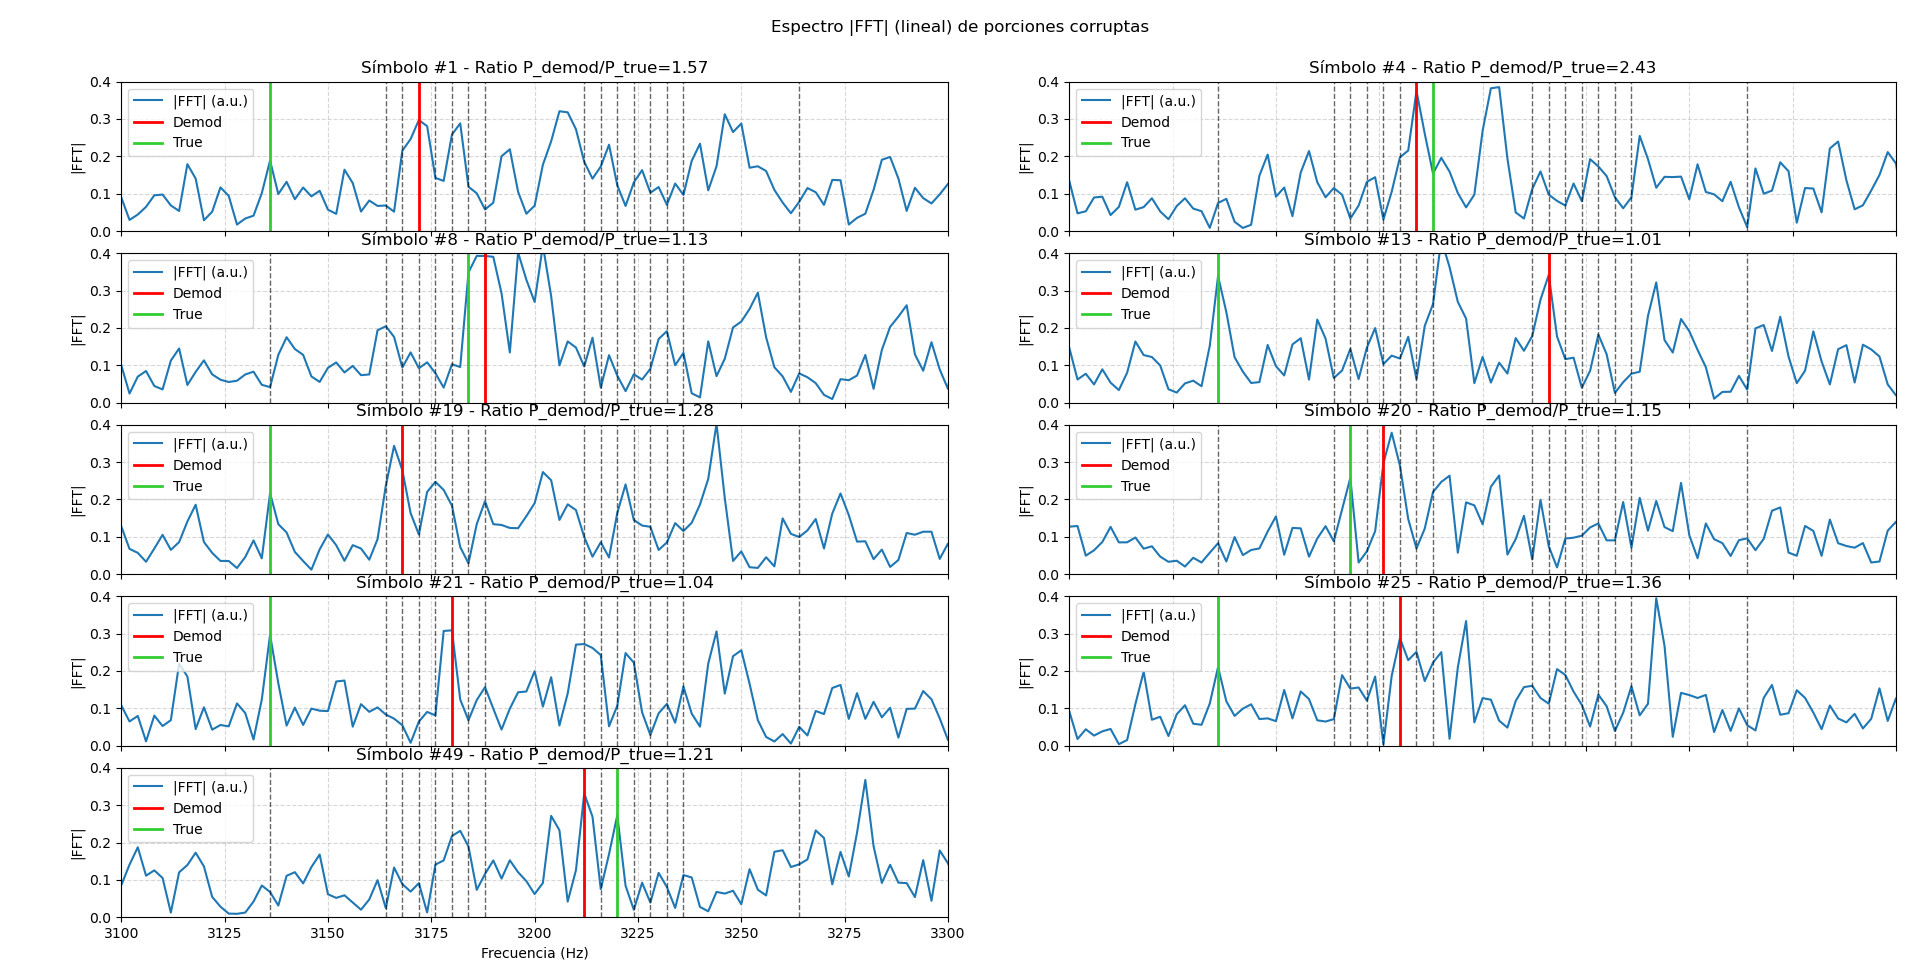
\includegraphics[width=0.9\textwidth]{img/mina/mal.png}
    \caption{Error in symbol demodulation at 120m in mine.}
    \label{fig:120m}
\end{figure}


It is possible to see that there were noise components with higher amplitude in comparison with the received tone signal. If we compare the noise distribution in mine and the noise in the astronomical observatory, we can see that in the mine, the noise is more impulsive and with higher amplitude and colored. \ref{fig:noisy}

\begin{figure}
    \centering
    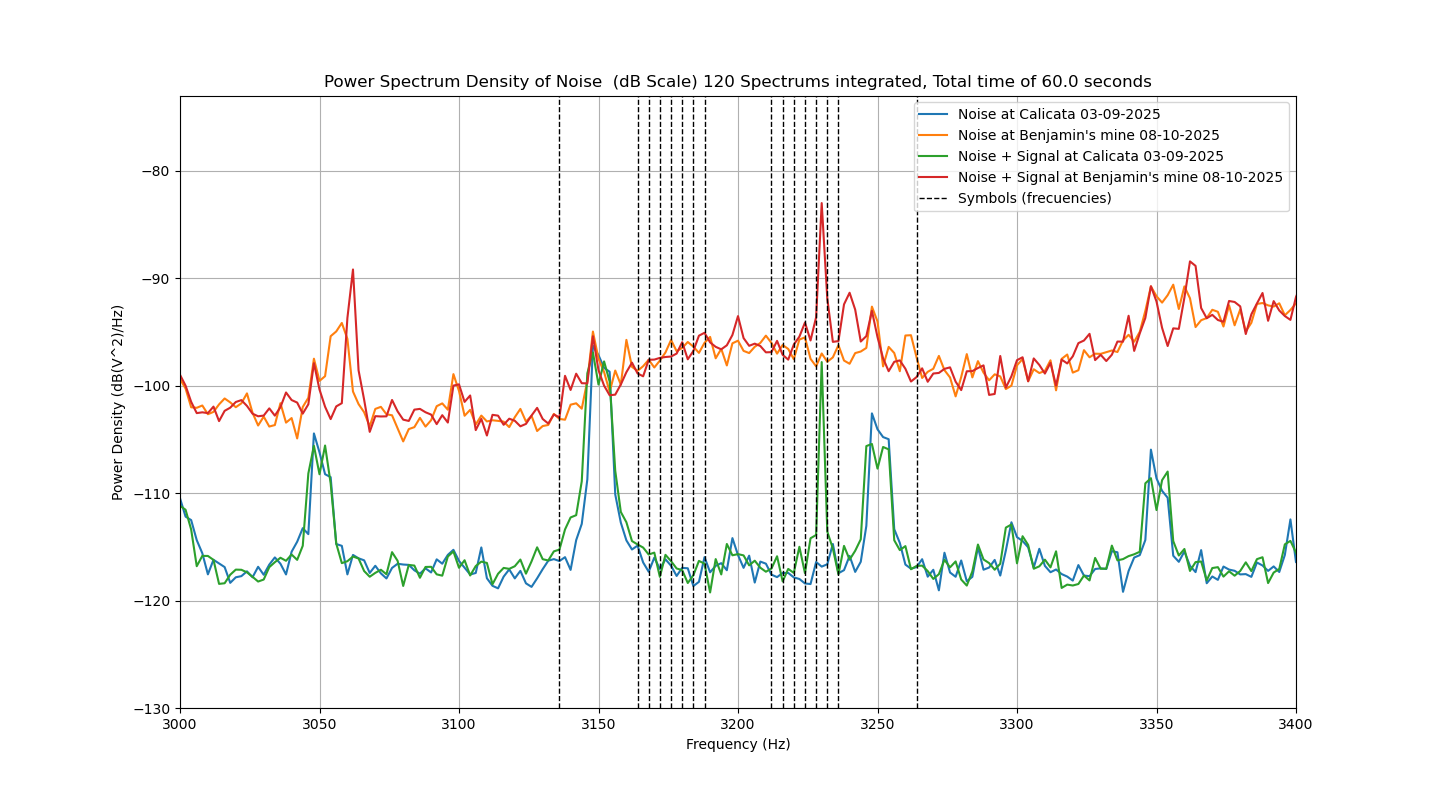
\includegraphics[width=0.9\textwidth]{img/ruidos_res_data_accumulada.png}
    \caption{Comparison of noise in mine and astronomical observatory (bottom).}
    \label{fig:noisy}
\end{figure}

This kind of noise affects the performance of the demodulator directly. After discounting the mean spectral distribution of noise, we could recover a certain amount of symbol demodulation as is shown in figure \ref{fig:120m-fixed}.

\begin{figure}
    \centering
    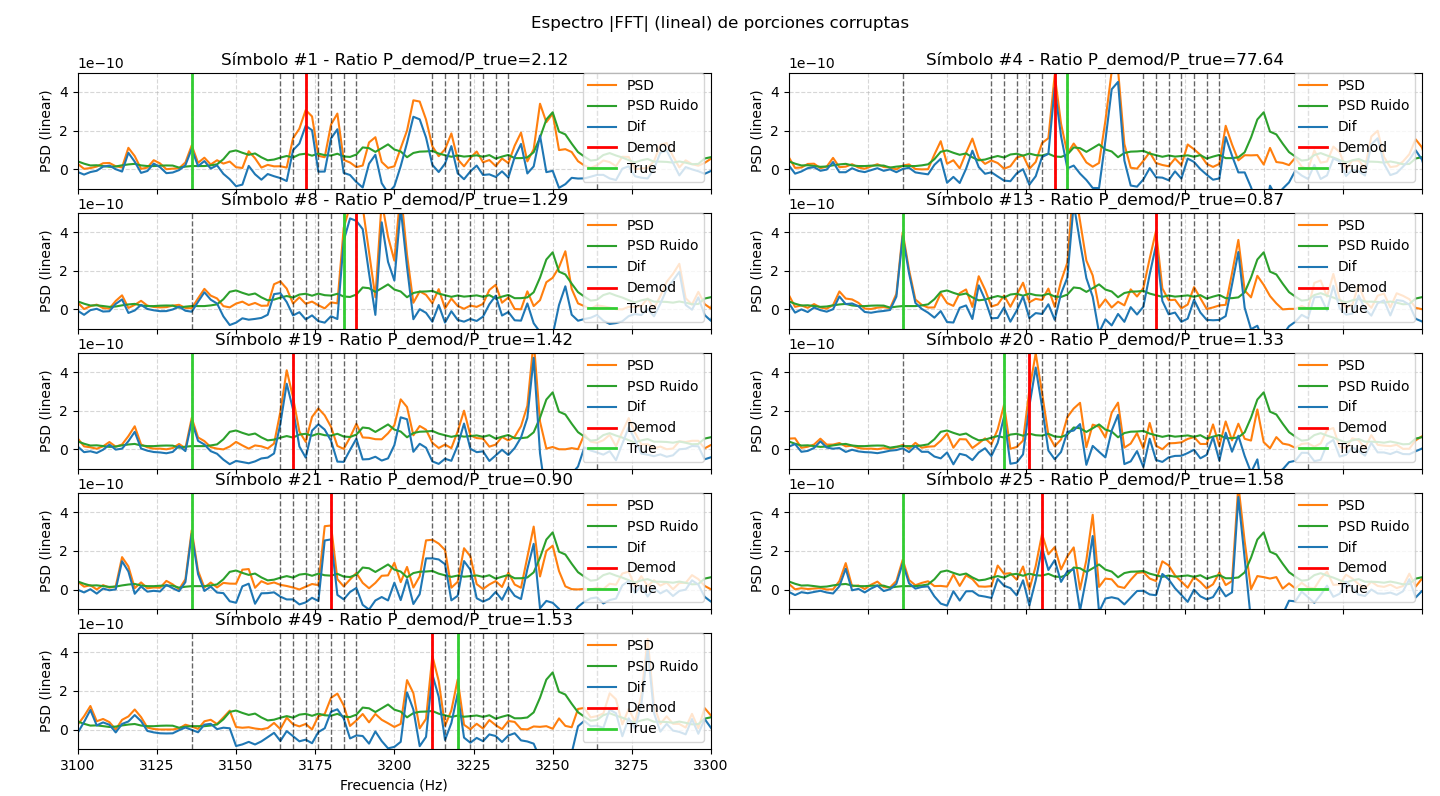
\includegraphics[width=0.9\textwidth]{img/mina/mejor.png}
    \caption{Error in symbol demodulation at 120m in mine after noise spectral subtraction.}
    \label{fig:120m-fixed}
\end{figure}

Although there is still a certain amount of error, this process allows us to understand better the characteristics of the underground channel in the mine and the kind of noise that affects the communication system. Finally, if we look at the temporal change of noise distribution at the mine, at figure \ref{fig:waterr} (inside the mine) and \ref{fig:waterrr} (outside the mine).

\begin{figure}
    \begin{subfigure}{0.9\textwidth}
        \centering
        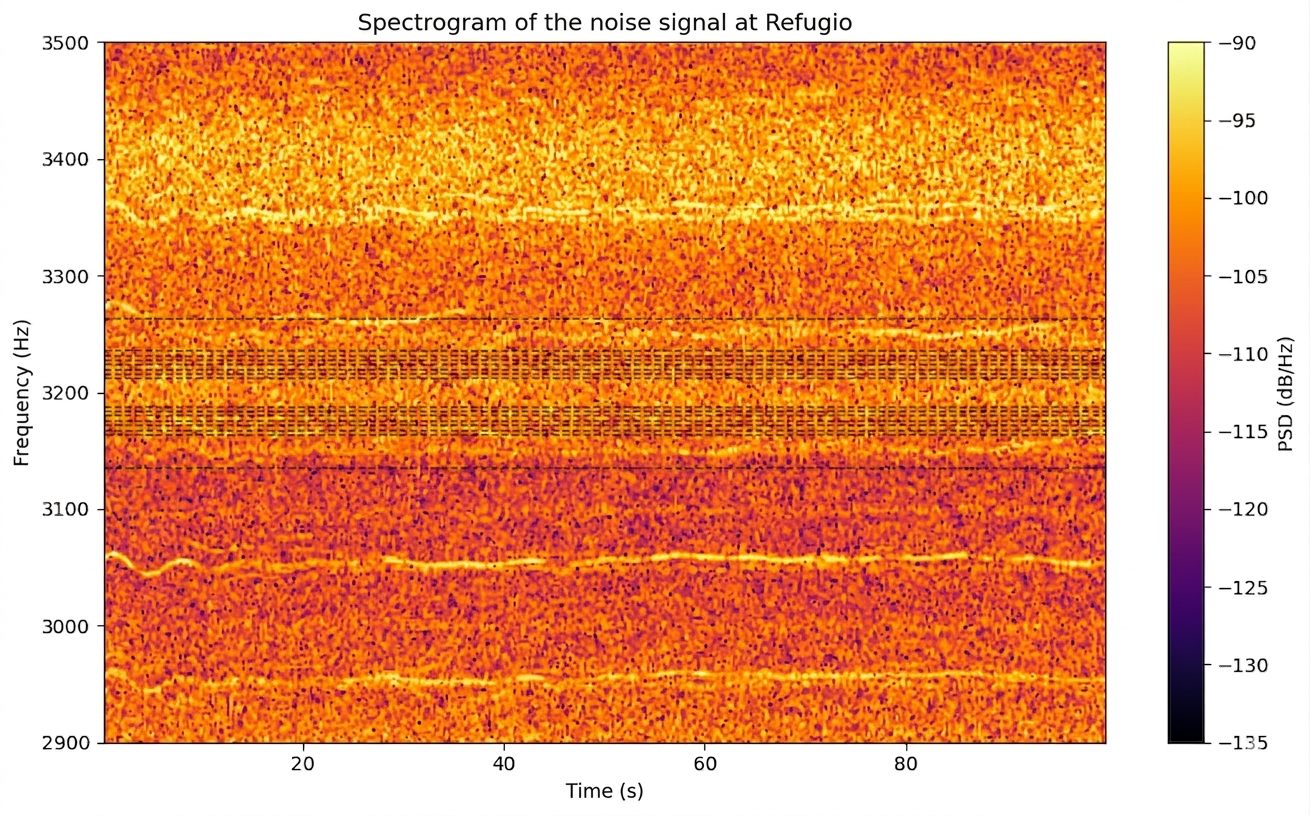
\includegraphics[width=\textwidth]{img/mina/refugioo.png}
        \caption{Temporal change of noise distribution at refuge, first level.}
        \label{fig:water1}
    \end{subfigure}
    \begin{subfigure}{0.9\textwidth}
        \centering
        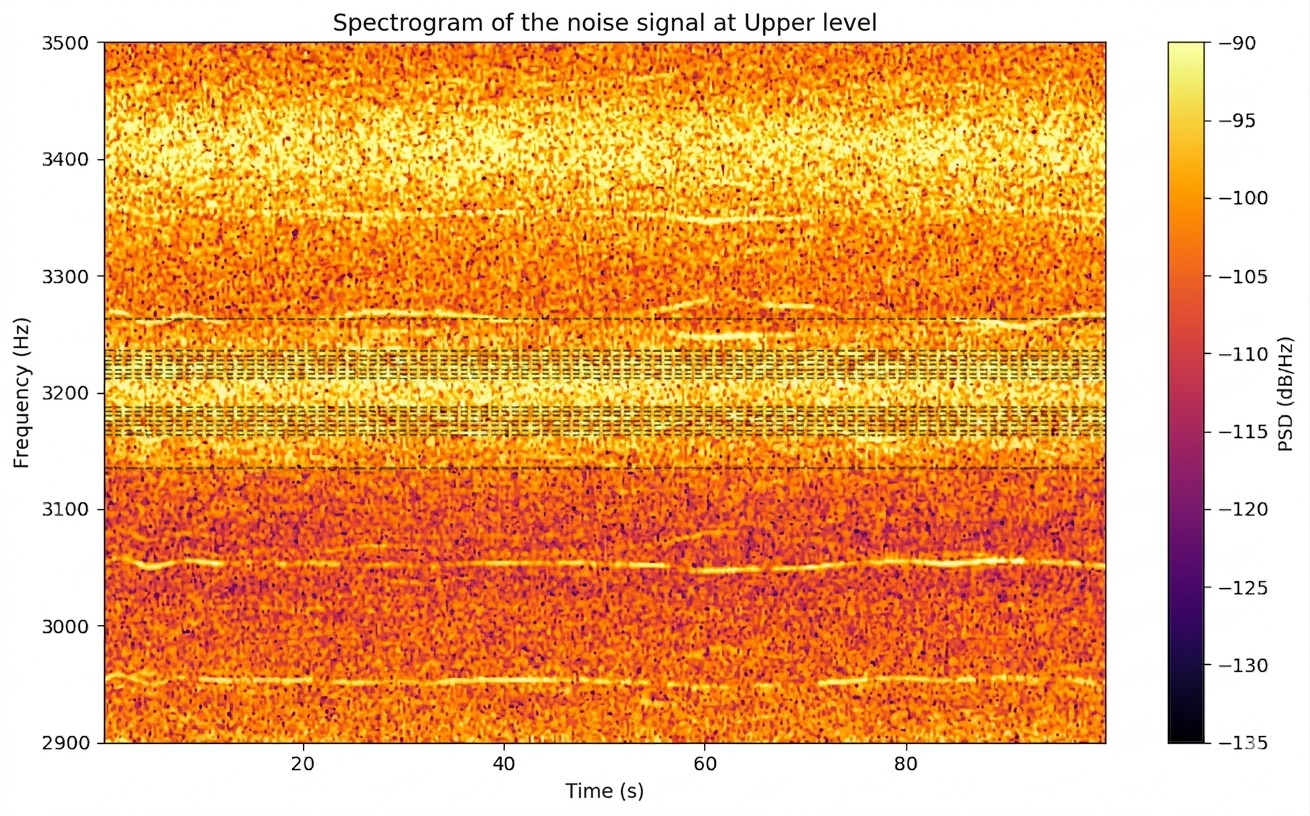
\includegraphics[width=\textwidth]{img/mina/upperlevel.png}
        \caption{Temporal change of noise distribution at superior level.}
        \label{fig:water2}
    \end{subfigure}
    \caption{Temporal change of noise distribution inside the mine.}
    \label{fig:waterr}
\end{figure}


\begin{figure}
    \begin{subfigure}{0.9\textwidth}
        \centering
        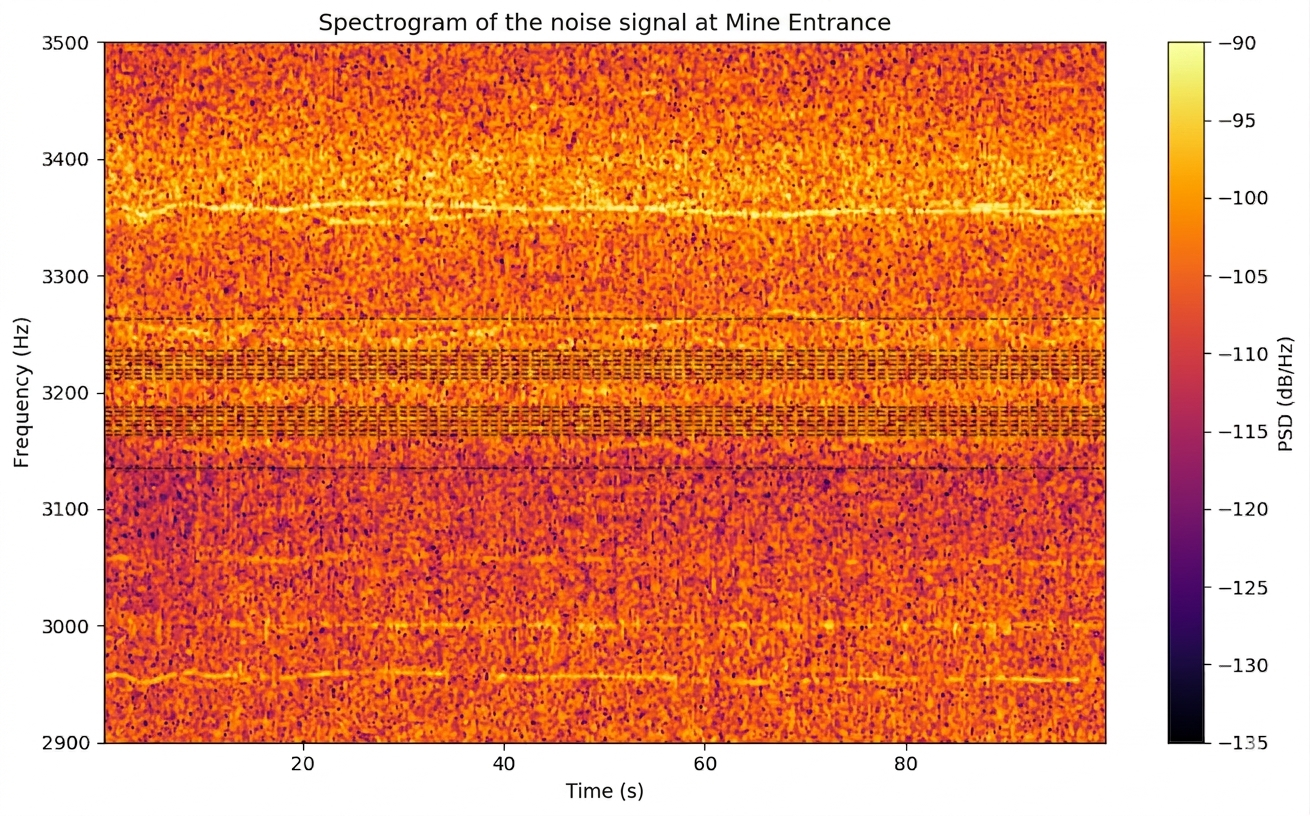
\includegraphics[width=\textwidth]{img/mina/mineentrance.png}
        \caption{Temporal change of noise distribution at entrance of the mine.}
        \label{fig:water3}
    \end{subfigure}
    \begin{subfigure}{0.9\textwidth}
        \centering
        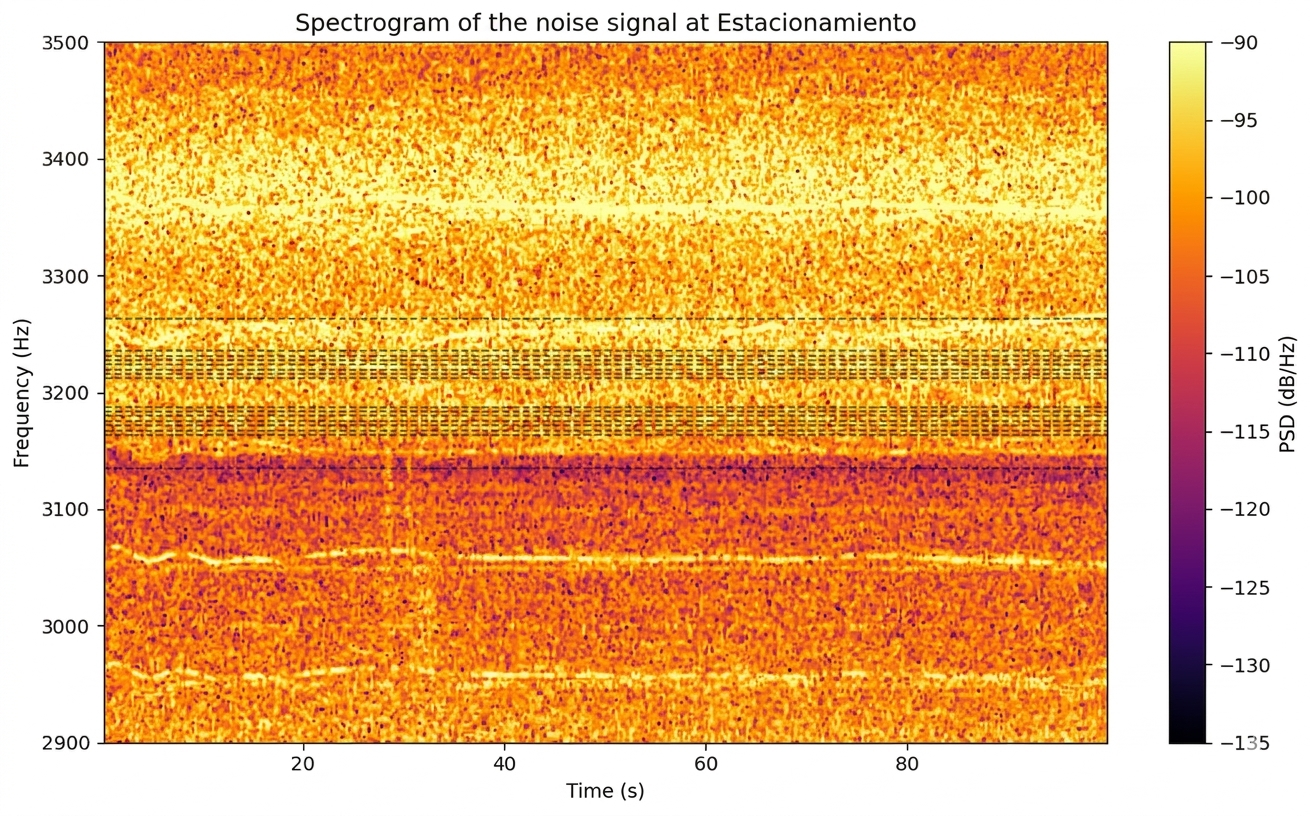
\includegraphics[width=\textwidth]{img/mina/esta.png}
        \caption{Temporal change of noise distribution at parking area.}
        \label{fig:water4}
    \end{subfigure}
    \caption{Temporal change of noise distribution outside the mine.}
    \label{fig:waterrr}
\end{figure}

\newpage

We can see that there are zones that are noisier than others, particularly at the system bandwidth (dashed black lines), places like the parking area outside the mine and the superior level inside the mine are pretty contaminated. At the 120 m test, the receiver was located at the refuge, and the messages were detected, but were not demodulated perfectly. When the receiver was in the parking area, almost all messages were corrupted. However, the detection works (correlation).
\newp
It's clear also that there exist noise sources in all places that are not constant in time, and those short-time interference affect the performance of the demodulation significantly. Also, there are noise sources that are more constant in time, which correspond to odd harmonics of the electrical grid. However, its frequency sometimes varies considerably.
\newp
It can be seen that there are more clean regions of the spectrum, for example, the band around 3100 $Hz$, but it is worth noticing that the analogical response of the coil is integrated in the perception of noise power.

\subsection{Field simulation for security}

An aspect not considered until now is the effect of MAGIC over other devices, i.e, MAGIC as an interference source. The magnetic field generated by the transmitter coil can induce currents in nearby conductive materials, which could potentially interfere with other electronic devices or pose safety risks to personnel. Regarding heavy machinery or other communication systems, MAGIC is not likely to cause significant interference due to the low power levels and the specific frequency range used. However, it is important to conduct a thorough analysis of the magnetic field generated and how it affects human health and medical devices, especially if the system is to be used in close proximity to personnel. A limit of 0.27 $\mu$T is defined as a safe exposure limit for the general public by the International Commission on Non-Ionizing Radiation Protection (ICNIRP) \cite{icnirp2010lf}. Here is a preliminary simulation of the magnetic flux density by the transmitter coil, considering a current of 3 A and a frequency of 3200 $Hz$, and the geometry of MAGIC's coil, shown in figures \ref{fig:Simulation_coil}. and \ref{fig:Simulation_coil_2}.

\begin{figure}
    \centering
    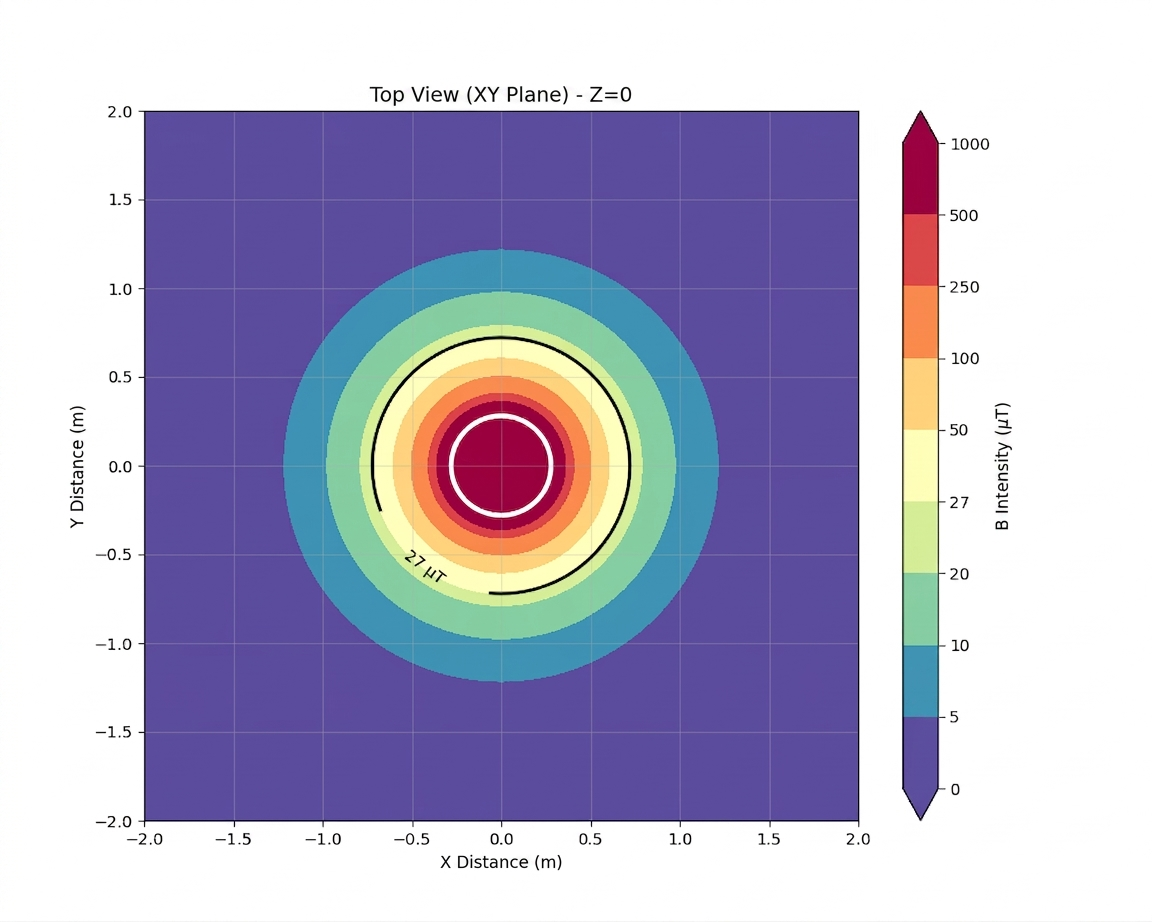
\includegraphics[width=0.7\textwidth]{img/diagrams/upper.png}
    \caption{Simulation of magnetic flux density generated by the transmitter coil, zenith view.}
    \label{fig:Simulation_coil}
\end{figure}

\begin{figure}
    \centering
    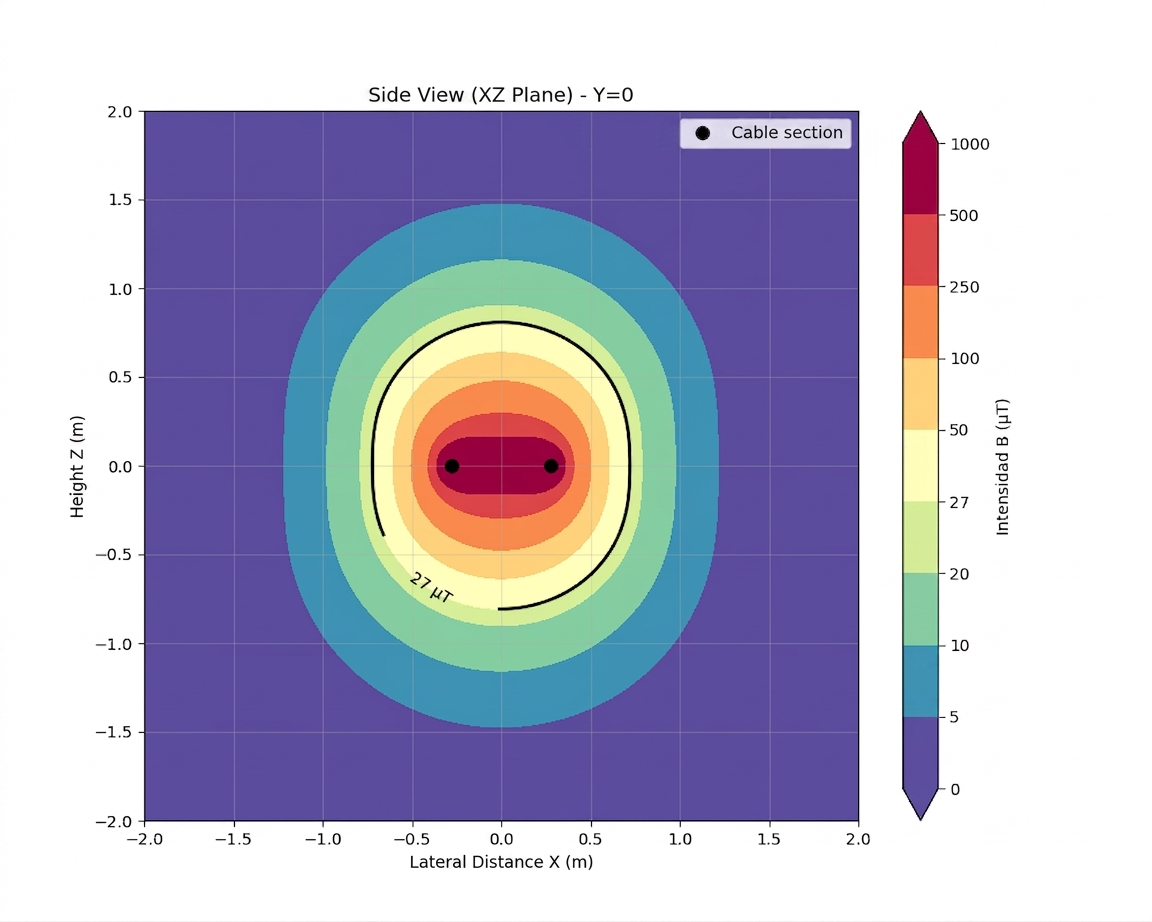
\includegraphics[width=0.7\textwidth]{img/diagrams/lat.png}
    \caption{Simulation of magnetic flux density generated by the transmitter coil, side view.}
    \label{fig:Simulation_coil_2}
\end{figure}

\subsection{Final Remarks}
Finally, the results obtained in the mine provide a lot of information about the characteristics of the underground environment with other types of rock composition, and the kind of noise that could affect the communication system. This information is crucial for future improvements of MAGIC.
\newp
Additionally, this experience in the mine provides valuable information about the conditions of operation and practical aspects to consider when implementing a communication system in a real mine.

 
